\section{Руководство пользователя}
\label{sec:guide}

Данное программное обеспечение призвано для упрощения процесса проведения функционального ТС КМУ артиллерийского
дивизиона.\break
Программное обеспечение используется в составе комплекса программ для автоматизации АРМ.
Комплекс программ устанавливается на все АРМ КМУ артиллерийского дивизиона.

В данном разделе приведено руководство оператора АРМ по использованию системы функционального контроля.
Руководство включает в себя требования к аппаратному и программному обеспечению, последовательность запуска, выполнения
и завершение программы функционального контроля, а также приведены сообщения, возникающие при функционировании программы
с указанием возможных команд по управлению процессом выполнения программы.

\subsection{Требования к аппаратному и программному обеспечению}
\label{sub:guide:reqs}

Так как разработанное ПО используется в составе комплекса программ для автоматизации АРМ, ниже приведены требования к
аппаратному и программному обеспечению для работы всего программного комплекса.

Программный комплекс устанавливается на ПЭВМ и бортовую ЭВМ.

ПЭВМ должна иметь следующие характеристики:
\begin{itemize}
	\item центральный процессор -- Intel Pentium с частотой не менее 1,90 ГГц;
	\item объем оперативной памяти -- 4 ГБ;
	\item объем накопителя на жестком диске, SSD -- не менее 256 ГБ;
	\item сетевой адаптер -- Ethernet 10/100/1000 Мбит/с;
	\item порт USB 2.0 -- 2 шт.;
	\item порт RS232/422/485 -- 4 шт.;
	\item порт DVI -- 1 шт.
\end{itemize}

Бортовая ЭВМ должна иметь следующие характеристики:
\begin{itemize}
	\item центральный процессор -- Intel с частотой не менее 1.6 ГГц;
	\item объем оперативной памяти -- не менее 4 ГБ;
	\item сенсорный экран -- размер не менее 10 дюймов (разрешение не менее 1280х800);
	\item объем накопителя на жестком диске, SSD -- не менее 240 ГБ;
	\item сетевой адаптер -- Ethernet 10/100/1000 Мбит/с не менее 2 шт.;
	\item порт USB 2.0 -- не менее 2 шт.;
	\item порт RS232 -- не менее 1 шт.
\end{itemize}

Для загрузки ПО требуется внешний привод DVD-ROM с возможностью подключения к порту USB.
В меню настроек BIOS компьютеров первым устройством должно быть установлено устройство чтения DVD -- ROM.
Программа функционального контроля функционирует в сети\break Ethernet с пропускной способностью 10/100/1000 Мбит/с.
Дополнительно для функционирования ПЭВМ должно быть установлено следующее периферийное оборудование:

\begin{itemize}
	\item принтер промышленный;
	\item видеомонитор;
	\item клавиатура;
	\item манипулятор графической информации.
\end{itemize}

Для функционирования программы функционального контроля должна быть установлена 64-разрядная
операционная система Windows 7\break Professional или Windows 7 Ultra.

\subsection{Установка программного обеспечения}
\label{sub:guide:intstallation}

Данное ПО предназначено для использования в составе программного комплекса по автоматизации АРМ КМУ
артиллерийского дивизиона.
Установка программного комплекса на ЭВМ КМУ артиллерийского дивизиона в данном разделе
рассмотрена не будет.

Для использования в тестовых и демонстрационных целях система\break функционального контроля может быть установлена и
использоваться отдельно от остального комплекса.
В этом случае для установки достаточно скопировать содержимое диска
с ПО на компьютер.

\subsection{Руководство по использованию системы}
\label{sub:guide:user_guide}

\subsubsection{Функциональный контроль технических средств}
\label{sub:guide:user_guide:func}
При использовании системы в составе программного комплекса, запуск программы осуществляется с помощью соответствующих
элементов графического интерфейса главного окна управляющей программы комплекса.

Запуск программы тестирования устройств
осуществляется запуском\break файла OfflinefunctionControl.exe, который находится в
подкаталоге bin каталога системы функционального контроля.
В результате запуска программы отобразится главное окно <<Функциональный контроль>> программы, приведенное на рис.
\ref{fig:guide:user_guide:func:main_window}.
\begin{figure}[htb]
	\centering
	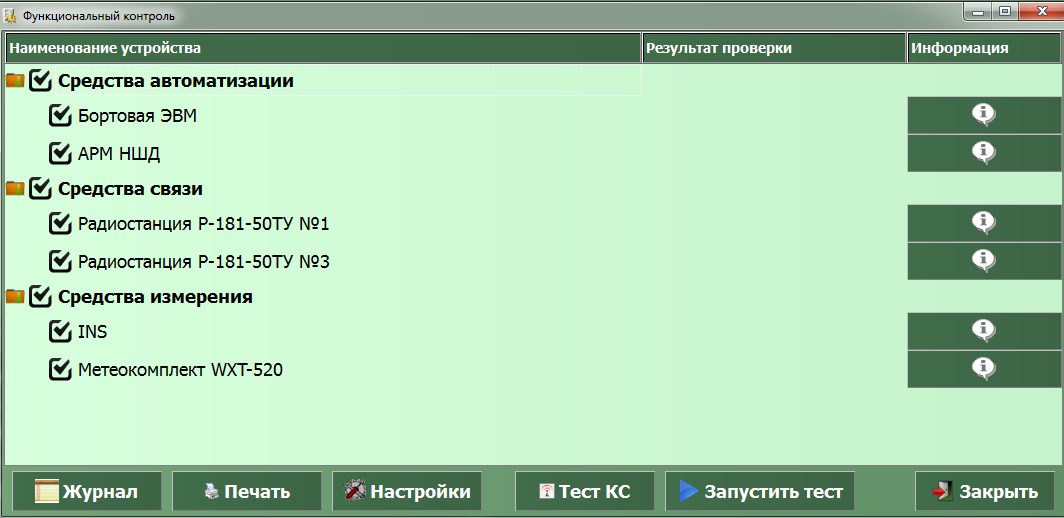
\includegraphics[scale=0.43]{main_window}
	\caption{Окно <<Функциональный контроль>>}
	\label{fig:guide:user_guide:func:main_window}
\end{figure}

Окно <<Функциональный контроль>> содержит список тестируемых технических средств
(наименование и количество устройств могут изменяться в зависимости от настроек АРМ).
Слева от наименования устройства имеется поле для установки флажка.
При нажатии кнопки <<Запустить тест>> запускаются тесты, отмеченные флажками.
При установке (снятии) флажка <<Средства автоматизации>>, <<Средства связи>>,
<<Средства измерения>> автоматически
устанавливаются (снимаются) флажки всех устройств, входящих в эту группу.
Тесты могут запускаться как по одному, так и все одновременно.
Результаты тестирования отображаются в столбце <<Результат проверки>> в виде сообщений:
\begin{itemize}
		\item <<Исправно>> (зеленого цвета);
		\item <<Неисправно>> (красного цвета);
		\item <<Порт занят>> (красного цвета).
\end{itemize}

При нажатии кнопки в столбце <<Информация>> открывается окно с подробной информацией о результатах проверки,
например, <<Бортовая ЭВМ>> (рис. \ref{fig:guide:user_guide:func:on_info}).
\begin{figure}
	\centering
	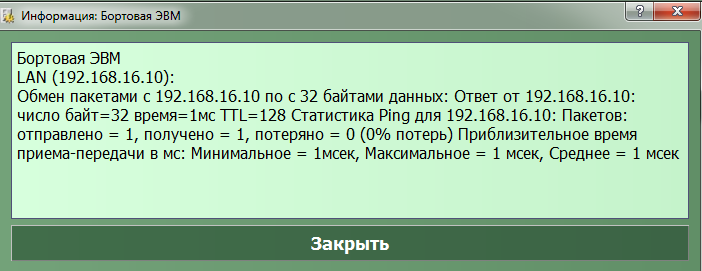
\includegraphics[scale=0.65]{on_info}
	\caption{Окно <<Информация: Бортовая ЭВМ>>}
	\label{fig:guide:user_guide:func:on_info}
\end{figure}
Для выхода из окна <<Информация: Бортовая ЭВМ>> нажать кнопку <<Закрыть>>.

По нажатию кнопки <<Настройки>> в окне <<Функциональный контроль>> (см.
рис.~\ref{fig:guide:user_guide:func:main_window}) отобразится окно <<Настройка АРМ>>, представленное на рис.
\ref{fig:guide:user_guide:func:on_settings}. Для настройки АРМ используется
программа, разработанная \company.
\begin{figure}
	\centering
	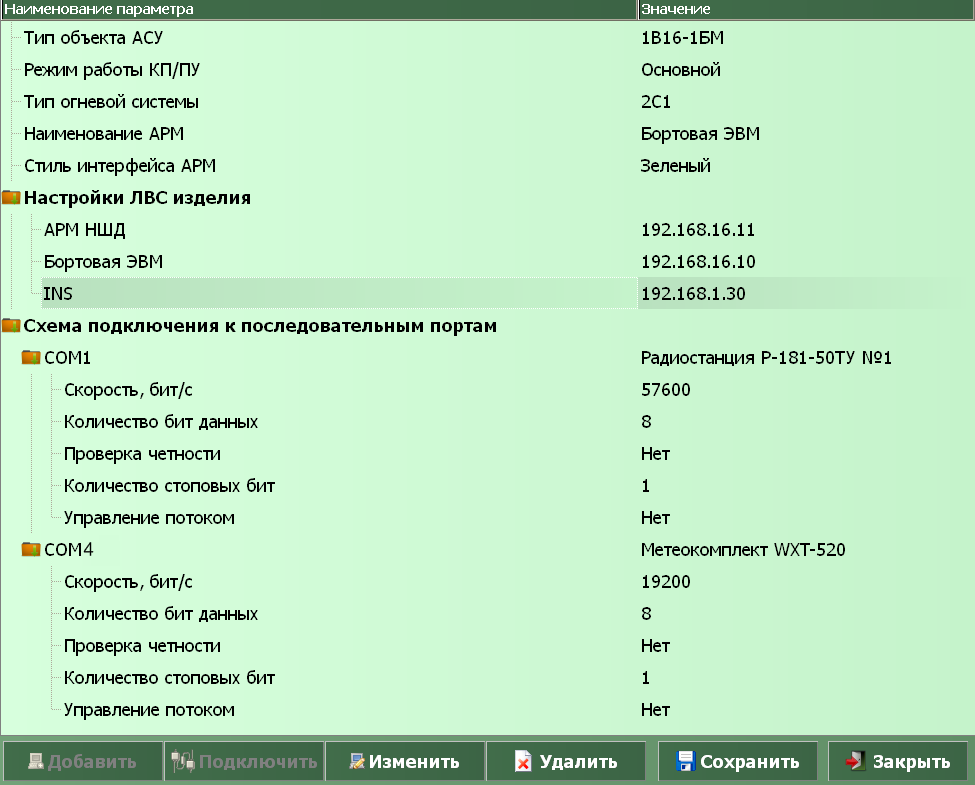
\includegraphics[scale=0.50]{on_settings}
	\caption{Окно <<Настройка АРМ>>}
	\label{fig:guide:user_guide:func:on_settings}
\end{figure}

По нажатию кнопки <<Печать>> в окне <<Функциональный контроль>>
(см. рис. \ref{fig:guide:user_guide:func:main_window}) формируется для просмотра и выдачи на принтер отчет
о проведенном функциональном контроле (рис. \ref{fig:guide:user_guide:func:on_print}).
\begin{figure}
	\centering
	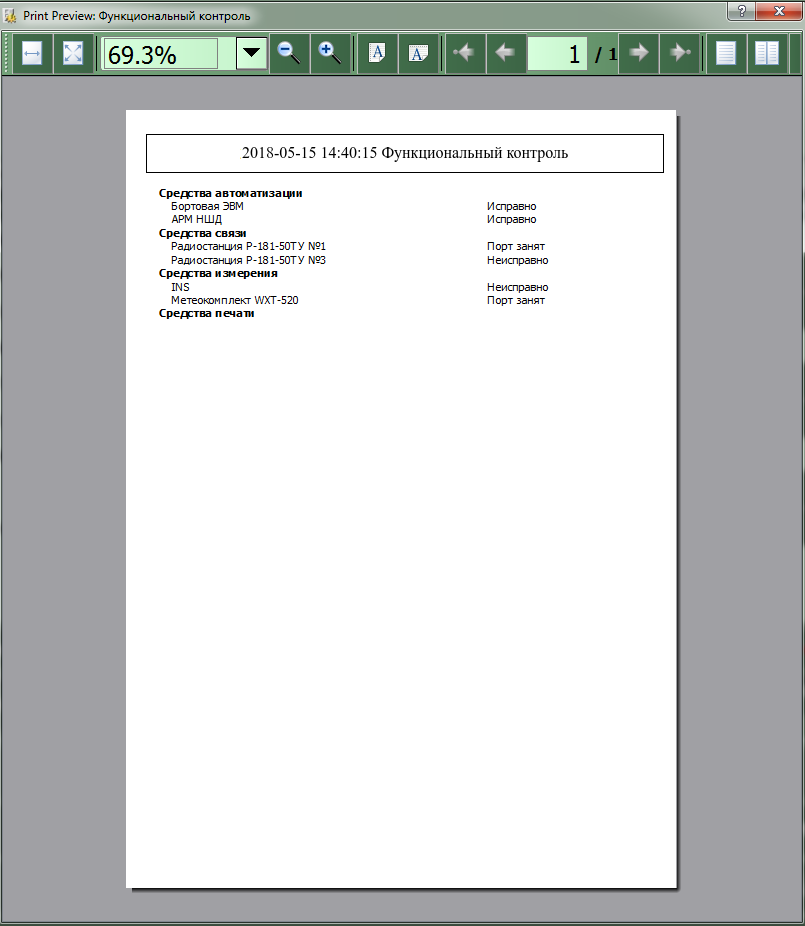
\includegraphics[scale=0.45]{on_print}
	\caption{Печать результатов тестирования}
	\label{fig:guide:user_guide:func:on_print}
\end{figure}

Выход из окна <<Функциональный контроль>> осуществляется по нажатию кнопки <<Закрыть>>.

\subsubsection{Тестирование каналов обмена данными}
\label{sub:guide:user_guide:radio}

Для тестирования каналов обмена данными необходимо нажать кнопку <<Тест КС>> (см. рис.
\ref{fig:guide:user_guide:func:main_window}).
В результате выполнения команды отобразится окно <<Тест каналов связи по радиостанциям Р–180/181>>, приведенное на рис.
\ref{fig:guide:user_guide:radio:on_test_cs}.
\begin{figure}[htb]
	\centering
	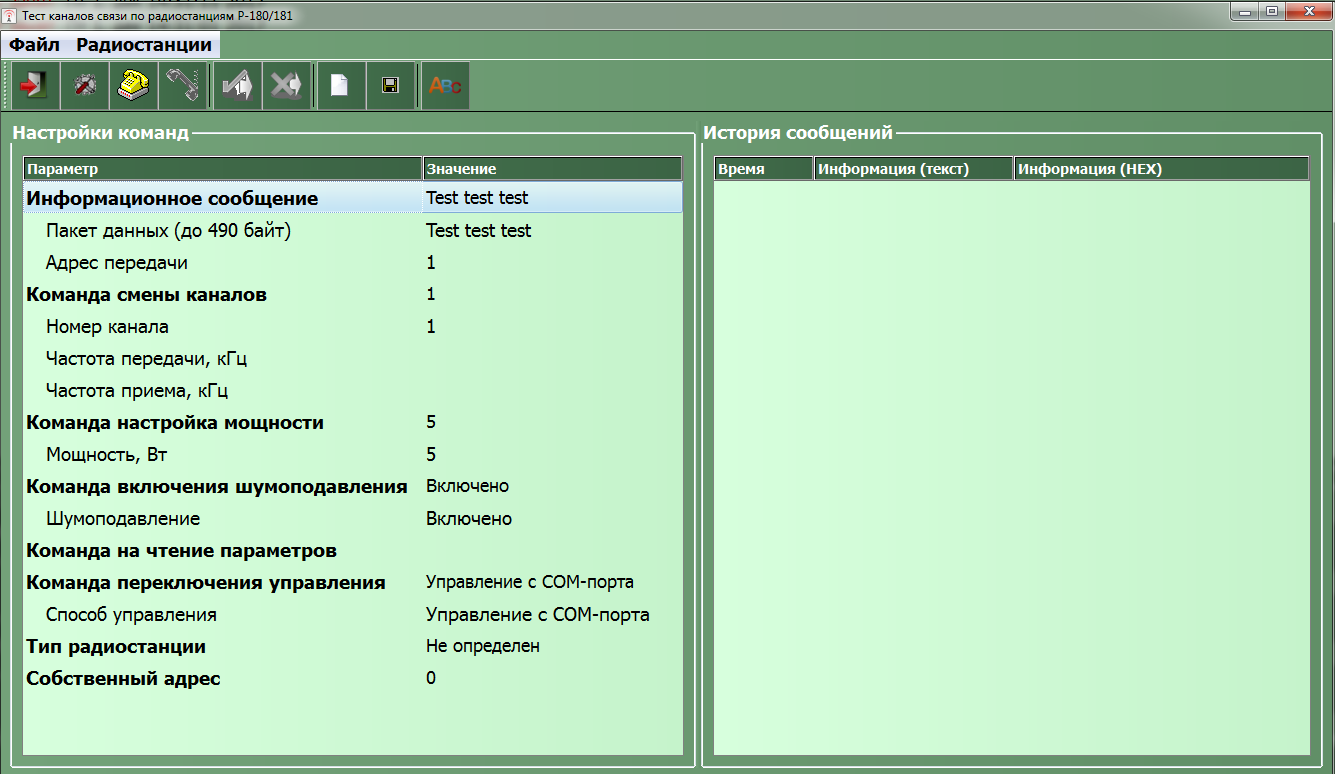
\includegraphics[scale=0.35]{on_test_cs}
	\caption{Окно <<Тест каналов связи по радиостанциям Р–180/181>>}
	\label{fig:guide:user_guide:radio:on_test_cs}
\end{figure}
В левой части окна (см. рис. \ref{fig:guide:user_guide:radio:on_test_cs}) отображается таблица <<Настройки команд>> с параметрами и значениями команд.
В правой части окна отображается таблица <<История сообщений>>, в которой хранится время получения сообщения.

В верхней части окна находится панель инструментов с кнопками, предназначенными для вызова требуемых функций.

Cлева направо на панели инструментов (см. рис. \ref{fig:guide:user_guide:radio:on_test_cs}) расположены\break кнопки:
\begin{itemize}
	\item <<Выход>>;
	\item <<Настройки>>;
	\item <<Открыть порт>>;
	\item <<Закрыть порт>>;
	\item <<Отправить сообщение>>;
	\item <<Очистить историю сообщений>>;
	\item <<Сохранить историю сообщений>>;
	\item <<Режим ввода>>.
\end{itemize}

В меню <<Файл>> могут выполняться следующие команды:
\begin{itemize}
	\item <<Настройки>>;
	\item <<Открыть порт>>;
	\item <<Закрыть порт>>;
	\item <<Показать историю сообщений>>;
	\item <<Сохранить историю сообщений>>;
	\item <<Выход>>.
\end{itemize}

В меню <<Радиостанции>> (см. рис.~\ref{fig:guide:user_guide:radio:on_test_cs}) выбирается тип используемой радиостанции.

При нажатии на кнопку <<Открыть порт>> на панели инструментов или выборе команды <<Открыть порт>> в меню <<Файл>> на радиостанцию выдается команда запроса параметров КС.

Для проверки канала связи необходимо выдать информационное сообщение, для чего нажать кнопку <<Отправить сообщение>> на
панели инструментов окна <<Тест каналов связи по радиостанциям Р–180/181>> (см.
рис.~\ref{fig:guide:user_guide:radio:on_test_cs}) или выполнить команду <<Отправить сообщение>> из контекстного меню.

Переданное сообщение отображается в таблице <<История сообщений>>, в которой отображаются и полученные сообщения от абонента.

Аналогично можно выдавать любое сообщение, изменяя его параметры. В информационном сообщении можно вводить любой текст,
размером 490 байт (символов). Кнопка <<Режим ввода>> (см. рис. ~\ref{fig:guide:user_guide:radio:on_test_cs}) служит для изменения режима ввода: текстовый или шестнадцатеричный.

После завершения проверки необходимо нажать кнопку <<Закрыть порт>> на панели инструментов (см.
рис.~\ref{fig:guide:user_guide:radio:on_test_cs}) или выполнить команду <<Закрыть порт>> из меню <<Файл>>.

Для настройки порта нажать кнопку <<Настройки>> на панели инструментов (см. рис. \ref{fig:guide:user_guide:radio:on_test_cs}) или выполнить команду
<<Настройки>> из меню <<Файл>>.
В результате выполнения команды отобразится окно, приведенное на рис. \ref{fig:guide:user_guide:radio:port_config}.
\begin{figure}[htb]
	\centering
	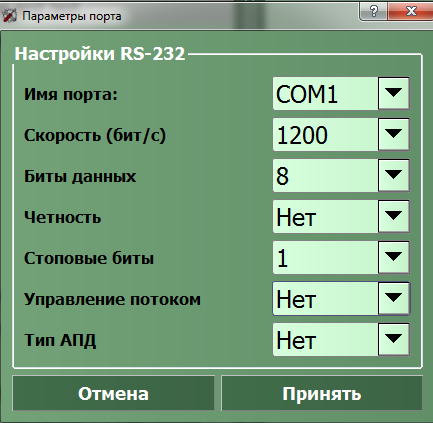
\includegraphics[scale=0.7]{port_config}
	\caption{Настройка параметров порта}
	\label{fig:guide:user_guide:radio:port_config}
\end{figure}
Поле <<Имя порта>>: -- редактируемое классификационное поле.

Поле <<Скорость (бит/с)>> -- редактируемое выбираемое целочисленное поле.

Поле <<Биты данных>> -- редактируемое выбираемое целочисленное поле.

Поле <<Четность>> -- редактируемое классификационное поле.

Поле <<Стоповые биты>> -- редактируемое выбираемое численное поле.

Поля <<Управление потоком>>, <<Тип АПД>> -- редактируемые классификационные поля.

Для сохранения настроек нажать кнопку <<Принять>>. Для отмены нажать кнопку <<Отмена>>.

При выборе команды <<Показать историю сообщений>> из меню <<Файл>> отобразится окно, приведенное на
рис.~\ref{fig:guide:user_guide:radio:on_test_cs}.
Для очистки таблицы <<История сообщений>> нужно нажать кнопку <<Очистить историю сообщений>> на панели инструментов (см.
рис.~\ref{fig:guide:user_guide:radio:on_test_cs}).
Для сохранения истории сообщений нажать кнопку <<Сохранить историю сообщений>> на панели инструментов окна <<Тест
каналов связи по радиостанциям Р–180/181>> (см. рис.~\ref{fig:guide:user_guide:radio:on_test_cs})  или выполнить команду
<<Сохранить историю сообщений>> из меню <<Файл>>.
Для выхода из окна <<Тест каналов связи по радиостанциям Р–180/181>> нажать кнопку <<Выход>> на панели инструментов (см.
рис.~\ref{fig:guide:user_guide:radio:on_test_cs}) или выполнить команду <<Выход>> из меню <<Файл>>.

\subsubsection{Использование журнала}
\label{sub:guide:user_guide:journal}
При нажатии кнопки <<Журнал>> в окне <<Функциональный контроль>>
(см. рис.~\ref{fig:guide:user_guide:func:main_window}) отобразится окно, приведенное на
рис.~\ref{fig:guide:user_guide:journal:journal_window}.

\begin{figure}[htb]
	\centering
	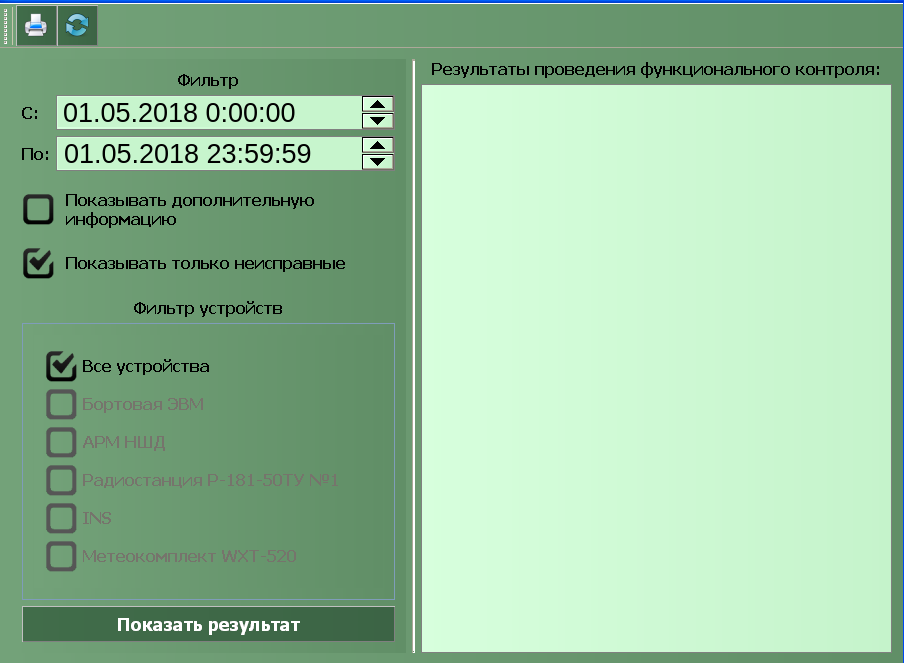
\includegraphics[scale=0.55]{journal_window}
	\caption{Окно <<Журнал тестирования ТС>>}
	\label{fig:guide:user_guide:journal:journal_window}
\end{figure}

В верхней части окна находится панель инструментов с кнопками, предназначенными для вызова требуемых функций.

Cлева направо на панели инструментов (см. рис.~\ref{fig:guide:user_guide:journal:journal_window}) расположены кнопки
(<<Обновить>>) и (<<Печать>>).

Для обновления информации в окне необходимо нажать кнопку <<Обновить>> на панели инструментов окна <<Журнал тестирования
ТС>>.

В левой части окна размещен фильтр, предназначенный для отображения определенной выборки сообщений
(рис.~\ref{fig:guide:user_guide:journal:journal_filters}).

\begin{figure}[!htb]
	\centering
	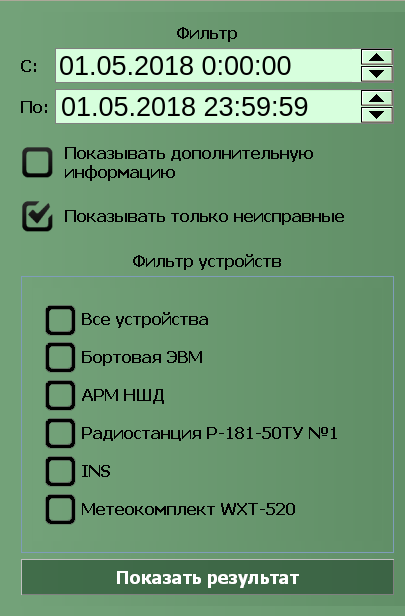
\includegraphics[scale=0.6]{journal_filters}
	\caption{Окно <<Журнал тестирования ТС>>}
	\label{fig:guide:user_guide:journal:journal_filters}
\end{figure}

Поля <<С:>>, <<По:>> – редактируемые временные поля.

Поля <<Показывать дополнительную информацию>>, <<Показывать только неисправные>> – выбираемые поля.

Поля из группы <<Фильтр устройств>> – выбираемые поля.

По нажатию кнопки <<Показать результат>> открывается окно, приведенное на
рис.~\ref{fig:guide:user_guide:journal:journal_items}, в котором отображаются результаты проведения функционального контроля
в соответствии с настроенным фильтром отображения информации.
\begin{figure}[h]
	\centering
	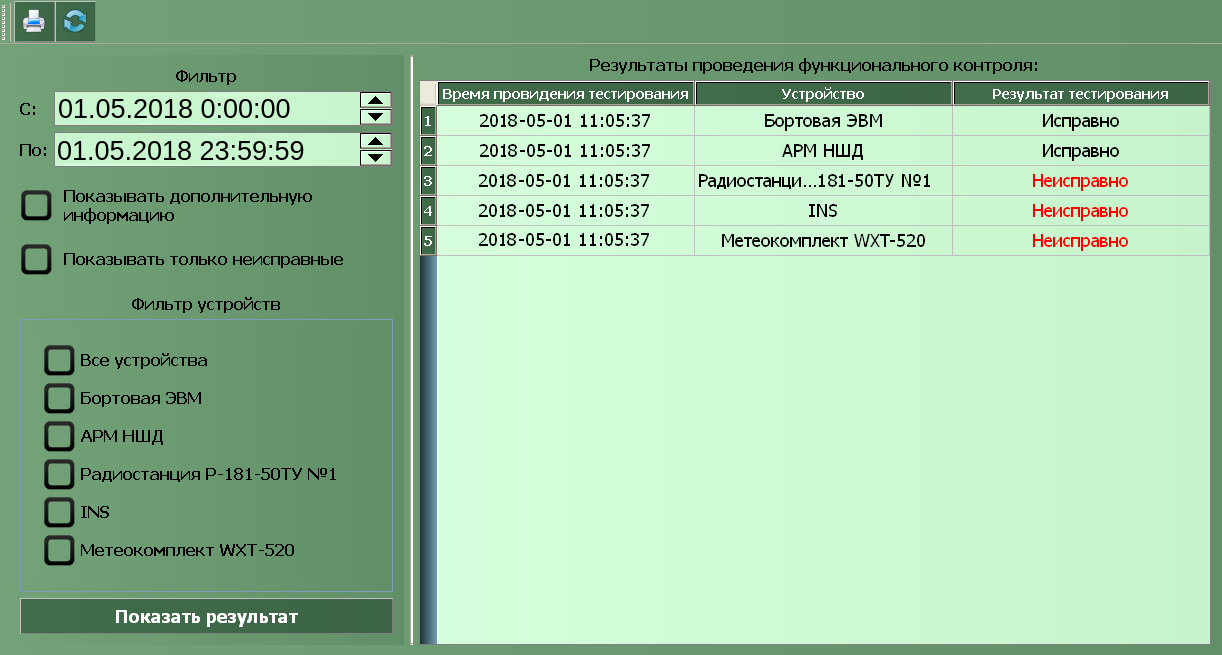
\includegraphics[scale=0.4]{journal_items}
	\caption{Результаты тестирования устройств}
	\label{fig:guide:user_guide:journal:journal_items}
\end{figure}

По нажатию кнопки <<Печать>> на панели инструментов формируется для просмотра и выдачи на принтер отчет о проведенном
функциональном контроле (рис.~\ref{fig:guide:user_guide:journal:journal_print}).
\begin{figure}[!htb]
	\centering
	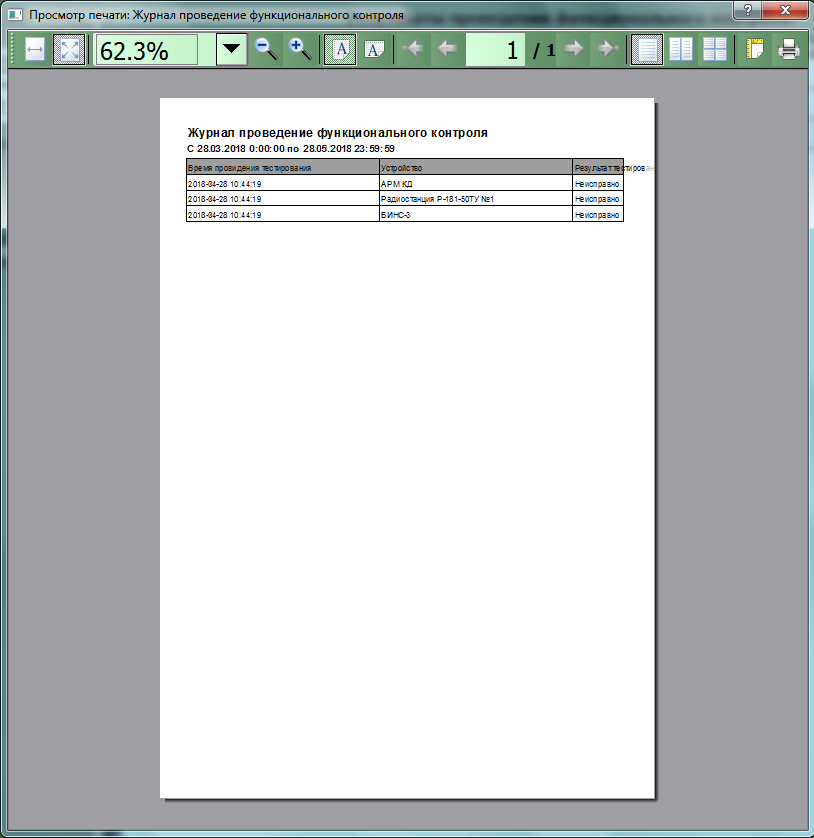
\includegraphics[scale=0.4]{journal_print}
	\caption{Печать страницы журнала}
	\label{fig:guide:user_guide:journal:journal_print}
\end{figure}

После нажатия кнопки <<Печать>> результаты тестирования печатаются на бумажном носителе.

